\documentclass[tikz,border=2pt,11pt]{standalone}
\usetikzlibrary{arrows.meta}
\usetikzlibrary{decorations.pathreplacing}
\usetikzlibrary{calc}
\usetikzlibrary{positioning}
\usepackage{amsmath}
\usepackage{amssymb}
\usepackage{graphicx}
\usepackage{xcolor}
\usepackage{tikz}
\newcommand{\R}{\mathbb R}
\newcommand{\Z}{\mathbb Z}
\newcommand{\N}{\mathbb N}
\newcommand{\F}{\mathbb F}
\newcommand{\E}{\mathbb E}
\newcommand{\Pp}{\mathbb P}
\newcommand{\one}{\mathbf 1}
\newcommand{\Id}{\mathrm{Id}}
\DeclareMathOperator{\TV}{TV}
\DeclareMathOperator{\supp}{supp}
\DeclareMathOperator{\rank}{rank}
\DeclareMathOperator{\diag}{diag}
\DeclareMathOperator{\Span}{span}
\DeclareMathOperator{\KL}{D}
\DeclareMathOperator{\dist}{dist}
\DeclareMathOperator{\diam}{diam}
\DeclareMathOperator{\Lip}{Lip}
\DeclareMathOperator{\tr}{tr}
\DeclareMathOperator{\osc}{osc}
\newcommand{\ip}[2]{\langle #1,#2\rangle}
\begin{document}
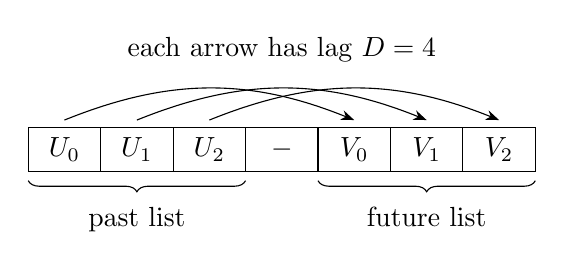
\begin{tikzpicture}[x=.92cm,y=1cm,>=Stealth]
 \foreach \j in {0,1,2,3,4,5,6}{
   \draw (\j,0) rectangle ++(1,.55);
 }
 \foreach \j in {0,1,2}{
   \node at (\j+.5,.275) {$U_{\j}$};
   \pgfmathtruncatemacro{\v}{\j+4}
   \node at (\v+.5,.275) {$V_{\j}$};
   \draw[->] (\j+.5,.65) to[bend left=22] (\v+.5,.65);
 }
 \node at (3.5,.275) {$-$};
 \draw[decorate,decoration={brace,mirror,amplitude=4pt}]
   (0,-.12)--(3,-.12) node[midway,below=6pt] {past list};
 \draw[decorate,decoration={brace,mirror,amplitude=4pt}]
   (4,-.12)--(7,-.12) node[midway,below=6pt] {future list};
 \node at (3.5,1.55) {each arrow has lag $D=4$};
\end{tikzpicture}
\end{document}
